\documentclass[xetex,mathserif,serif]{beamer}
\usepackage{polyglossia}
\setdefaultlanguage[babelshorthands=true]{russian}
\usepackage{minted}
\usepackage{tabu}

\useoutertheme{infolines}

\usepackage{fontspec}
\setmainfont{FreeSans}
\newfontfamily{\russianfonttt}{FreeSans}

\setbeamertemplate{blocks}[rounded][shadow=false]
\setbeamercolor*{block title example}{fg=green!50!black,bg=green!20}
\setbeamercolor*{block body example}{fg=black,bg=green!10}

\setbeamercolor*{block title alerted}{fg=red!50!black,bg=red!20}
\setbeamercolor*{block body alerted}{fg=black,bg=red!10}

\tabulinesep=0.7mm

\title{Программирование на платформе .NET}
\subtitle{Введение, основы C\#}
\author[Юрий Литвинов]{Юрий Литвинов \newline \textcolor{gray}{\small\texttt{yurii.litvinov@gmail.com}}}

\date{1}

\begin{document}
	
	\frame{\titlepage}
	
	\begin{frame}
		\frametitle{О курсе}
		\begin{itemize}
			\item Рассказ про основные языки для .NET --- C\# и (немного) F\#
			\item Немного про саму платформу
			\item Будет также про основные библиотеки и технологии (WinForms, WPF, MVC, EF и т.д.)
			\item Лекции (каждую неделю), семинары (не каждую неделю), домашние задания
			\item Оценка: домашние задания (70\%), экзамен в конце курса (30\%)
		\end{itemize}
	\end{frame}

	\begin{frame}
		\frametitle{Язык C\#}
		\begin{itemize}
			\item Объектно-ориентированный язык общего назначения с сильной типизацией
			\item Основной язык программирования для платформы .NET
			\item Первая версия --- 2002 год, актуальная --- 07.03.2017, C\# 7.0
			\item Международный стандарт (ISO/IEC 23270:2006)
			\item В основном для прикладного ПО
			\item 5-е место в индексе TIOBE
			\item Работает под Windows (.NET, .NET Core) и Linux/Mac OS (Mono, .NET Core)
			\item Средства разработки:
			\begin{itemize}
				\item Rider (\url{https://www.jetbrains.com/rider/})
				\item Microsoft Visual Studio (\url{https://www.visualstudio.com})
				\item MonoDevelop (\url{http://www.monodevelop.com/})
				\item Visual Studio Code (\url{https://code.visualstudio.com/})
			\end{itemize}
		\end{itemize}
	\end{frame}

	\begin{frame}
		\frametitle{Common Language Infrastructure}
		\begin{columns}
			\begin{column}{0.5\textwidth}
				\begin{small}
					\begin{itemize}
						\item Компиляция в байткод виртуальной машины (Common Intermediate Language, CIL)
						\item Виртуальная машина и набор библиотек (Common Language Runtime) реализуется для каждой платформы (ОС)
						\item Машина интерпретирует байт-код или компилирует его <<на лету>> в машинные коды
						\item Прежде всего для облегчения разработки компиляторов и обеспечения взаимодействия языков
					\end{itemize}
				\end{small}
			\end{column}
			\begin{column}{0.5\textwidth}
				\begin{center}
					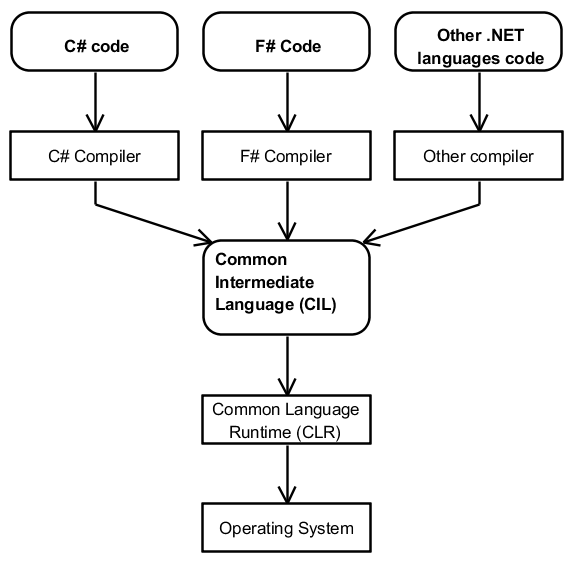
\includegraphics[width=\textwidth]{CLI.png}
				\end{center}
			\end{column}
		\end{columns}
	\end{frame}

	\begin{frame}
		\frametitle{Байт-код}
		Дизассемблер JetBrains dotPeek:
		\begin{center}
			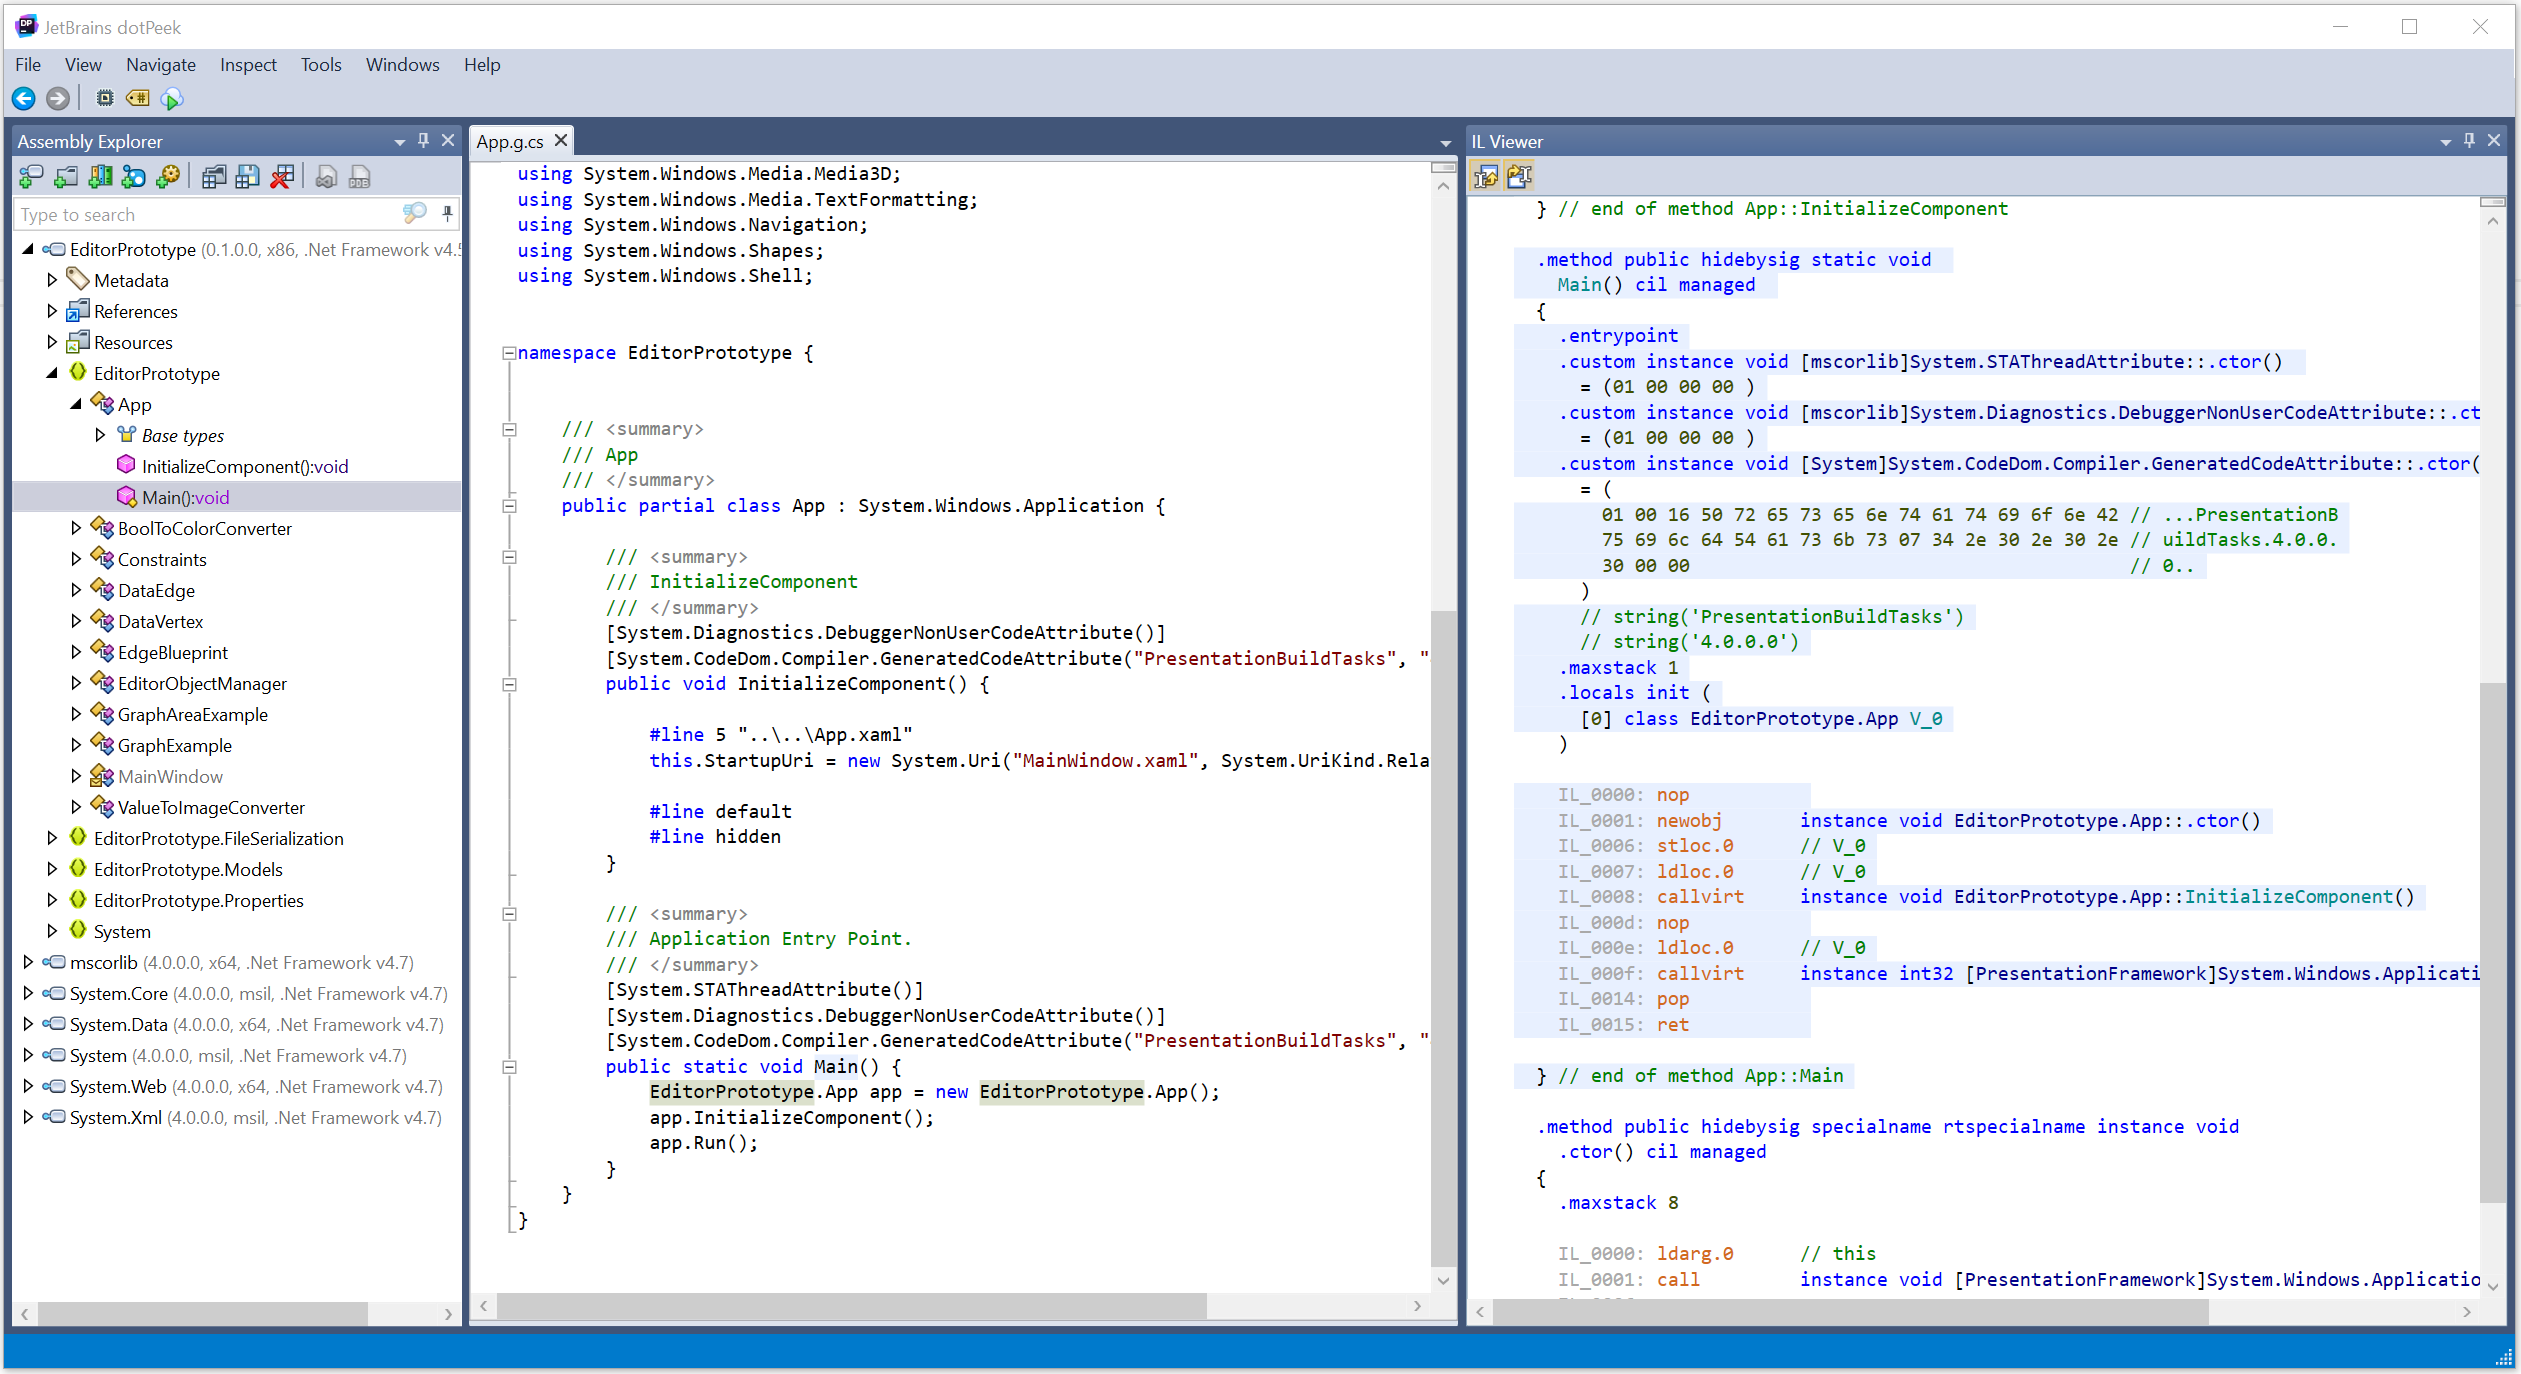
\includegraphics[width=0.8\textwidth]{dotPeek.png}
		\end{center}
		Ещё есть ildasm.exe
	\end{frame}

	\begin{frame}[fragile]
		\frametitle{Технические подробности C\#}
		\framesubtitle{Как обычно, Hello, World}
		\begin{minted}{csharp}
using System;

namespace HelloWorld
{
    class Program
    {
        static void Main(string[] args)
        {
            Console.WriteLine("Goodbye, cruel world!");
        }
    }
}
		\end{minted}
\end{frame}

	\begin{frame}[fragile]
		\frametitle{Циклы}
		\begin{minted}{csharp}
for (int i = 0; i < 300; ++i)
{
    Console.WriteLine("Hello, world!");
}
		\end{minted}
		или
		\begin{minted}{csharp}
for (var i = 0; i < 300; ++i)
{
    Console.WriteLine("Hello, world!");
}
		\end{minted}
\end{frame}

	\begin{frame}[fragile]
		\frametitle{Методы}
		\begin{minted}{csharp}
private static int Factorial(int n)
{
    if (n <= 1)
    {
         return 1;
    }

    return n * Factorial(n - 1);
}
		\end{minted}
		или так:
		\begin{minted}{csharp}
private static int Factorial(int n) 
    => n <= 1 ? 1 : n * Factorial(n - 1);
		\end{minted}
\end{frame}

	\begin{frame}
		\frametitle{Стайлгайд}
		\begin{itemize}
			\item \href{https://msdn.microsoft.com/en-us/library/ff926074.aspx}{C\# Coding Conventions}
			\item \href{https://stylecop.codeplex.com/}{https://stylecop.codeplex.com/}
			\begin{itemize}
				\item \href{https://github.com/DotNetAnalyzers/StyleCopAnalyzers}{https://github.com/DotNetAnalyzers/StyleCopAnalyzers}
			\end{itemize}
			\item \href{https://msdn.microsoft.com/en-us/library/3z0aeatx.aspx}{Code Analysis for Managed Code (бывший FxCop)}
		\end{itemize}
	\end{frame}

	\begin{frame}
		\frametitle{Элементарные типы}
		\begin{itemize}
			\item Всё --- объект, даже \mintinline{csharp}|int| наследуется от \mintinline{csharp}|Object|
			\item Типы стандартизованы: размер и множество значений одинаковы во всех реализациях
			\item Каждому типу соответствует библиотечный класс
			\begin{itemize}
				\item Например, \mintinline{csharp}|int| --- \mintinline{csharp}|System.Int32|
			\end{itemize}
			\item У каждого типа есть значение по умолчанию
			\begin{itemize}
				\item Им переменные и поля инициализируются при создании
				\item Ключевое слово \mintinline{csharp}|default|, особо полезно в генериках
			\end{itemize}
		\end{itemize}
	\end{frame}

	\begin{frame}[fragile]
		\frametitle{Методы у типов}
		\begin{minted}{csharp}
var inputString = Console.ReadLine();
int number = int.Parse(inputString);
		\end{minted}
		--- это то же самое, что
		\begin{minted}{csharp}
var inputString = Console.ReadLine();
int number = Int32.Parse(inputString);
		\end{minted}
\end{frame}

	\begin{frame}[fragile]
		\frametitle{Массивы}
		\begin{minted}{csharp}
int[] a = new int[10];
		\end{minted}
		или
		\begin{minted}{csharp}
var a = new int[10];
		\end{minted}
		Пример:
		\begin{minted}{csharp}
for (var i = 0; i < a.Length; ++i)
{
    a[i] = i;
}
		\end{minted}
		Двумерные массивы:
		\begin{minted}{csharp}
int[,] numbers = new int[3, 3];
numbers[1, 2] = 2; 
int[,] numbers2 = new int[3, 3] { {2, 3, 2}, {1, 2, 6}, {2, 4, 5} };
		\end{minted}
\end{frame}

	\begin{frame}[fragile]
		\frametitle{Перечисления}
		Объявление:
		\begin{minted}{csharp}
enum SomeEnum
{
        red,
        green,
        blue
}
		\end{minted}
		Использование:
		\begin{minted}{csharp}
SomeEnum a = SomeEnum.blue;
		\end{minted}
		(ну или через \mintinline{csharp}|var|: \mintinline{csharp}|var a = SomeEnum.blue;|)
\end{frame}

	\begin{frame}[fragile]
		\frametitle{Структуры}
		\begin{minted}{csharp}
struct Point
{
    public int x;
    public int y;
}
		\end{minted}
		\begin{itemize}
			\item Тип-значение
			\item Может содержать поля, методы, конструкторы и т.д.
			\item Не может иметь конструктор без параметров
			\item Может быть создан без вызова конструктора
			\item Может реализовывать интерфейсы
			\item Не может наследоваться
		\end{itemize}
\end{frame}

	\begin{frame}
		\frametitle{Ссылочные типы и типы-значения}
		Ссылочные типы:
		\begin{itemize}
			\item Классы
			\item Строки
			\item Массивы
			\item Исключения
			\item Делегаты
		\end{itemize}
		Типы-значения:
		\begin{itemize}
			\item Примитивные типы
			\item Перечисления
			\item Структуры
		\end{itemize}
	\end{frame}

	\begin{frame}[fragile]
		\frametitle{Пример}
		\begin{minted}{csharp}
static void Add(string s1, string s2, string s3)
{
    s3 = s1 + s2;
}
		\end{minted}
\end{frame}

	\begin{frame}[fragile]
		\frametitle{Передача параметров по ссылке}
		\begin{minted}{csharp}
static void Add(string s1, string s2, ref string s3)
{
    s3 = s1 + s2;
}

private static void Main(string[] args)
{
    string s1 = "a";
    string s2 = "b";
    string s3 = "c";
    Add(s1, s2, ref s3);
}
		\end{minted}
\end{frame}

	\begin{frame}[fragile]
		\frametitle{Out-параметры}
		\begin{minted}{csharp}
static void Add(string s1, string s2, out string s3)
{
    s3 = s1 + s2;
}

private static void Main(string[] args)
{
    string s1 = "a";
    string s2 = "b";
    Add(s1, s2, out string s3);
    Console.WriteLine(s3);
}
		\end{minted}
\end{frame}

	\begin{frame}[fragile]
		\frametitle{Кортежи и декомпозиция}
		\begin{minted}{csharp}
static (int prev, int cur) Fibonacci(int n)
{
    var (prevPrev, prev) = n <= 2 ? (0, 1) : Fibonacci(n - 1);
    return (prev, prevPrev + prev);
}

private static void Main(string[] args)
{
    var (_, result) = Fibonacci(7);
    Console.WriteLine(result);
}
		\end{minted}
\end{frame}

	\begin{frame}[fragile]
		\frametitle{Конструкторы}
		\begin{minted}{csharp}
class Circle
{
    public Circle(int x, int y, int r)
    {
        this.x = x;
        this.y = y;
        this.r = r;
    }

    private int x;
    private int y;
    private int r;
}
		\end{minted}
\end{frame}

	\begin{frame}[fragile]
		\frametitle{Перегрузка конструкторов, chaining}
		\begin{small}
			\begin{minted}{csharp}
class Circle
{
    public Circle(int x, int y, int r)
    {
        this.x = x;
        this.y = y;
        this.r = r;
    }

    public Circle(int r)
        : this(0, 0, r)
    {
    }

    private int x;
    private int y;
    private int r;
}
			\end{minted}
		\end{small}
\end{frame}

	\begin{frame}[fragile]
		\frametitle{Наследование (1)}
		\begin{minted}{csharp}
class Shape
{
    public Shape()
    {
    }

    public Shape(int x, int y)
    {
        this.x = x;
        this.y = y;
    }

    protected int x;
    protected int y;
}
		\end{minted}
\end{frame}

	\begin{frame}[fragile]
		\frametitle{Наследование (2)}
		\begin{minted}{csharp}
class Circle : Shape
{
    Circle(int x, int y, int r)
    {
        this.x = x;
        this.y = y;
        this.r = r;
    }

    Circle(int r)
        : base(0, 0)
    {
    }

    private int r;
}
		\end{minted}
\end{frame}

	\begin{frame}[fragile]
		\frametitle{Интерфейсы}
		\begin{minted}{csharp}
interface IDrawable
{
    void Draw();
}
		\end{minted}
\end{frame}

	\begin{frame}[fragile]
		\frametitle{Реализация интерфейса}
		\begin{minted}{csharp}
class Shape : IDrawable
{
    public void Draw()
    {
        Console.Write("Drawing Shape");
    }

    protected int x;
    protected int y;
}
		\end{minted}
\end{frame}

	\begin{frame}[fragile]
		\frametitle{Явная реализация интерфейса}
		\begin{minted}{csharp}
class Shape : IDrawable
{
    void IDrawable.Draw()
    {
        Console.Write("Drawing Shape");
    }

    protected int x;
    protected int y;
}
		\end{minted}
\end{frame}

	\begin{frame}[fragile]
		\frametitle{Абстрактные классы}
		\begin{minted}{csharp}
abstract class Shape
{
    public Shape() 
    {
    }

    public abstract void Draw();

    protected int x;
    protected int y;
}
		\end{minted}
\end{frame}

	\begin{frame}[fragile]
		\frametitle{Виртуальные методы (1)}
		\begin{minted}{csharp}
class Shape
{
    public virtual void Draw()
    {
        Console.WriteLine(
                "Drawing Shape with coords ({0}, {1})", x, y);
    }

    protected int x;
    protected int y;
}
		\end{minted}
\end{frame}

	\begin{frame}[fragile]
		\frametitle{Виртуальные методы (2)}
		\begin{minted}{csharp}
class Circle : Shape
{
    public Circle(int x, int y, int r)
    {
        this.x = x;
        this.y = y;
        this.r = r;
    }

    public override void Draw()
    {
        Console.WriteLine("Drawing Circle with radius {0}", r);
    }

    private int r;
}
		\end{minted}
\end{frame}

	\begin{frame}[fragile]
		\frametitle{Виртуальные методы (3)}
		\begin{footnotesize}
			\begin{minted}{csharp}
class Rectangle : Shape
{
    public Rectangle(int x, int y, int width, int height)
    {
        this.x = x;
        this.y = y;
        this.width = width;
        this.height = height;
    }
    public override void Draw()
    {
        base.Draw();
        Console.WriteLine(
            "Drawing Rectangle with width={0} and height={1}", width, height);
    }
    protected int width;
    protected int height;
}
			\end{minted}
		\end{footnotesize}
\end{frame}

	\begin{frame}[fragile]
		\frametitle{Виртуальные методы (4)}
		\begin{minted}{csharp}
private static void Main(string[] args)
{
    var circle = new Circle(0, 0, 10);
    var rectangle = new Rectangle(0, 0, 10, 10);
    var list = new System.Collections.Generic.List<Shape>();
    list.Add(circle);
    list.Add(rectangle);
    foreach (var shape in list)
    {
        shape.Draw();
    }
}
		\end{minted}
\end{frame}

	\begin{frame}[fragile]
		\frametitle{Абстрактные методы}
		\begin{minted}{csharp}
abstract class Shape
{
    public abstract void Draw();

    protected int x;
    protected int y;
}
		\end{minted}
\end{frame}

	\begin{frame}[fragile]
		\frametitle{Перевведение методов, new (1)}
		\begin{minted}{csharp}
class Shape
{
    public virtual void Draw()
    {
        Console.WriteLine(
                "Drawing Shape with coords ({0}, {1})", x, y);
    }

    protected int x;
    protected int y;
}
		\end{minted}
\end{frame}

	\begin{frame}[fragile]
		\frametitle{Перевведение методов, new (2)}
		\begin{small}
			\begin{minted}{csharp}
class Circle : Shape
{
    public Circle(int x, int y, int r)
    {
        this.x = x;
        this.y = y;
        this.r = r;
    }

    public new void Draw()
    {
        Console.WriteLine("Drawing Circle with radius {0}", r);
    }

    private int r;
}
			\end{minted}
		\end{small}
\end{frame}

	\begin{frame}[fragile]
		\frametitle{Перевведение методов, new (3)}
		\begin{minted}{csharp}
Circle circle1 = new Circle(10, 10, 3);
Shape circle2 = new Circle(10, 10, 3);
var circle3 = new Circle(10, 10, 3);

circle1.Draw();
circle2.Draw();
circle3.Draw();
		\end{minted}
\end{frame}

	\begin{frame}
		\frametitle{Модификаторы видимости}
		\begin{itemize}
			\item \mintinline{csharp}|public| --- применяется к типам и членам, доступ без ограничений
			\item \mintinline{csharp}|protected| --- применяется только к членам, доступ в типе и потомках
			\item \mintinline{csharp}|internal| --- применяется к типам и членам, доступ внутри сборки
			\item \mintinline{csharp}|protected internal| --- применяется к типам и членам, доступ внутри сборки \textbf{или} в потомках
			\item \mintinline{csharp}|private| --- применяется к типам и членам, доступ только внутри типа
			\item По умолчанию для типов \mintinline{csharp}|internal|, для членов --- \mintinline{csharp}|private|
		\end{itemize}
	\end{frame}

	\begin{frame}
		\frametitle{Другие модификаторы}
		\begin{itemize}
			\item \mintinline{csharp}|partial| --- <<частичный>> класс, декларирует, что определение класса разбито на несколько файлов
			\begin{itemize}
				\item Для интеграции сгенерированного и рукописного кода, не используйте без нужды
			\end{itemize}
			\item \mintinline{csharp}|sealed| --- запрещение наследования от класса
			\item \mintinline{csharp}|static| --- не может быть инстанцирован, может содержать только \mintinline{csharp}|static|-методы
		\end{itemize}
	\end{frame}

	\begin{frame}[fragile]
		\frametitle{Вложенные классы}
		\begin{footnotesize}
			\begin{minted}{csharp}
class Circle
{
    private readonly Point pos;
    private readonly int r;

    private class Point
    {
        public int x;
        public int y;
    }

    public Circle(int x, int y, int r)
    {
        pos = new Point {x = 10, y = 10};
        this.r = r;
    }

    public void Draw() =>
        Console.WriteLine($"({pos.x}, {pos.y}), radius {r}");
}
			\end{minted}
		\end{footnotesize}
\end{frame}

	\begin{frame}[fragile]
		\frametitle{Преобразования типов}
		\begin{minted}{csharp}
Shape shape = new Circle();
Circle circle = (Circle)shape;

Shape shape = new Circle();
Circle circle = shape as Circle;

Shape shape = new Circle();
if (shape is Circle)
{
    Circle circle = (Circle)shape;
}
		\end{minted}
\end{frame}

\end{document}

